
\begin{figure}[H]
    \centering
    \label{figure:margins}
    \begin{subfigure}[H]{1\textwidth}
    \centering
    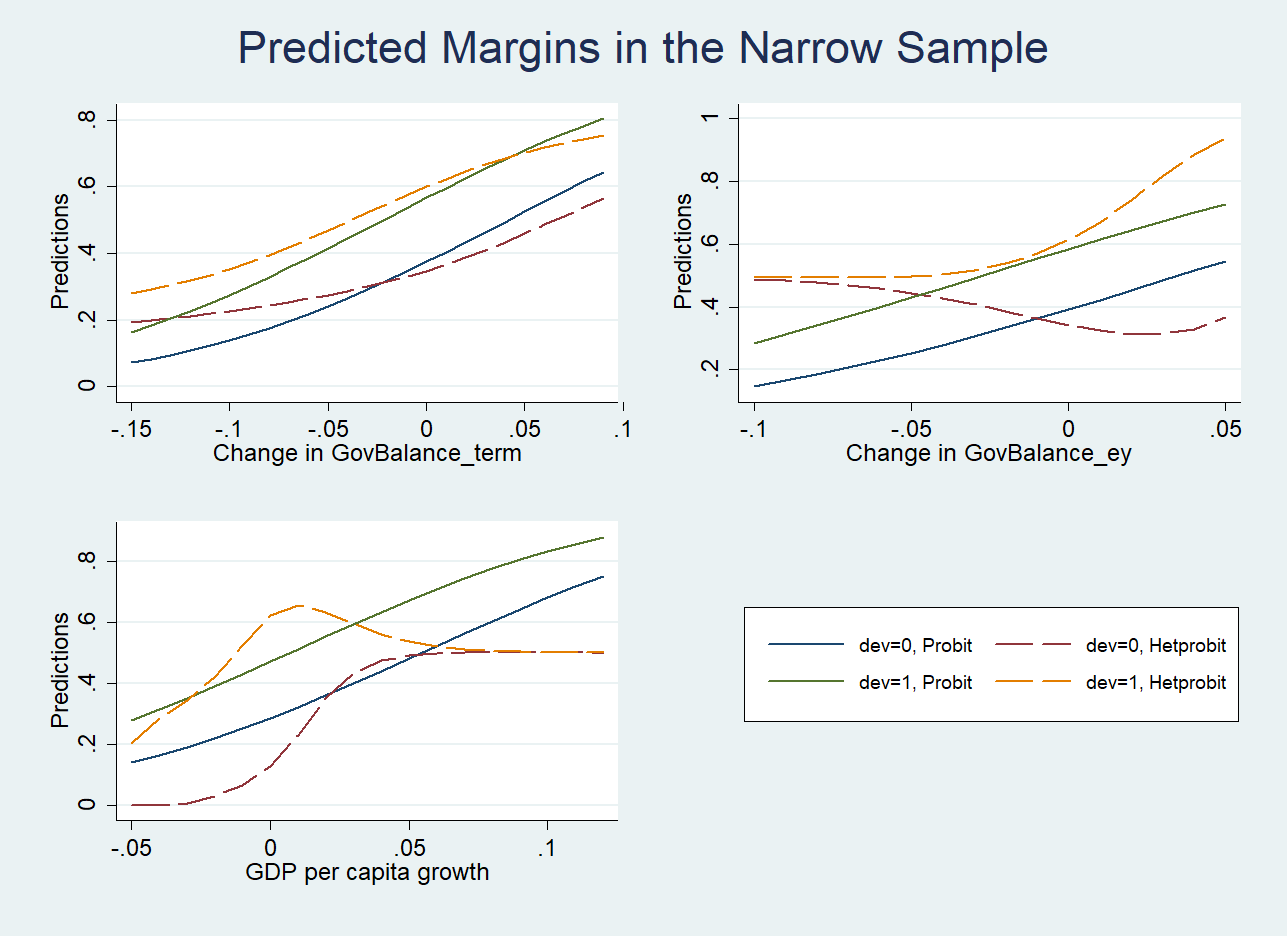
\includegraphics[width=0.8\textwidth]{Predicted_Narrow.png}
    \end{subfigure}
    \begin{subfigure}[H]{1\textwidth}
    \centering
    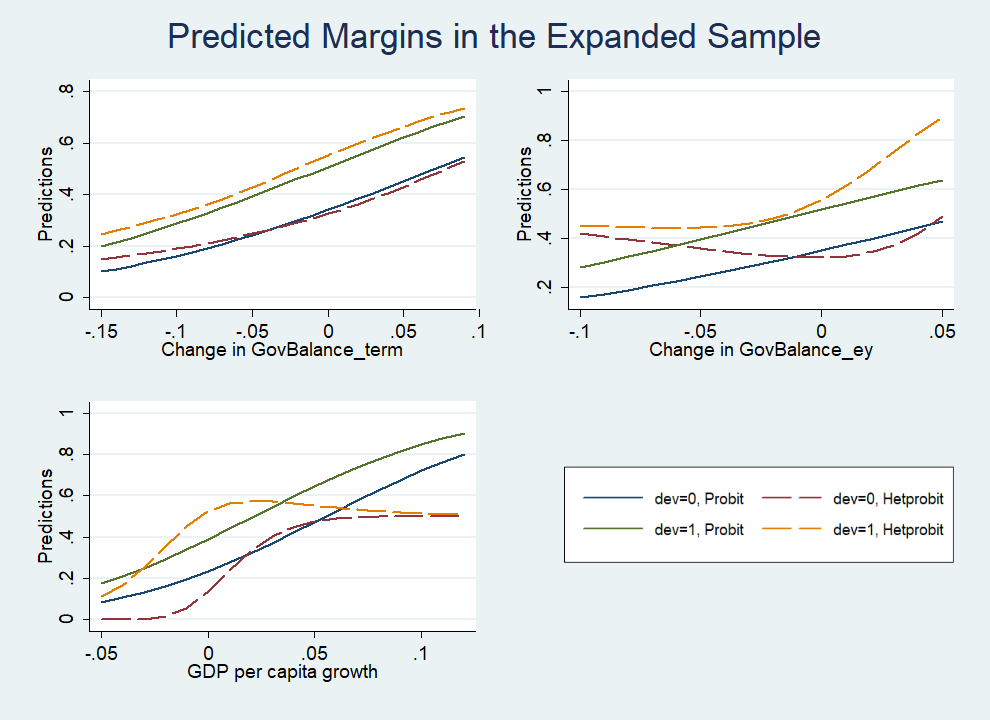
\includegraphics[width=0.8\textwidth]{Predicted_Expanded.png}
    \end{subfigure}
    \caption{\small{Predicted margins of the regular Probit (solid lines) and Heteroskedastic Probit model (dashed lines) for both Developed and Less Developed countries. Variables displayed are: the change in Government Balance over the leader's term, change in Government Balance in the election year and GDP per capita growth rate}}
    \label{Predicted_Narrow}
\end{figure}
\begin{figure}[H]
    \centering
    \label{figure:marginal effects}
        \begin{subfigure}[H]{1\textwidth}
    \centering
    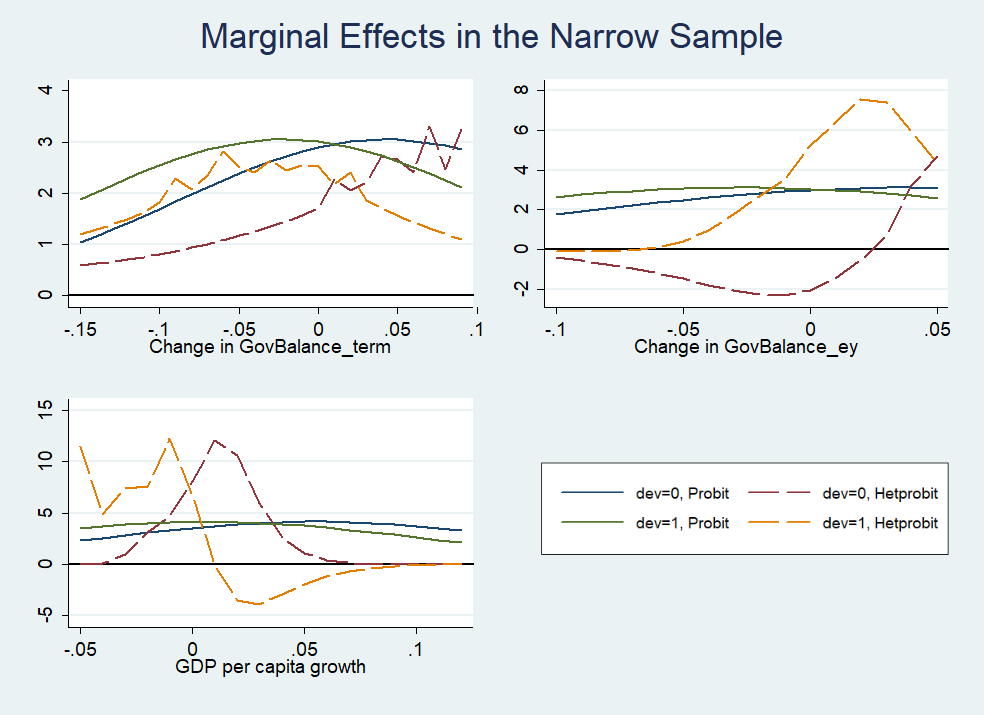
\includegraphics[width=0.8\textwidth]{AME_Narrow.png}
    \end{subfigure}
    \begin{subfigure}[H]{1\textwidth}
    \centering
    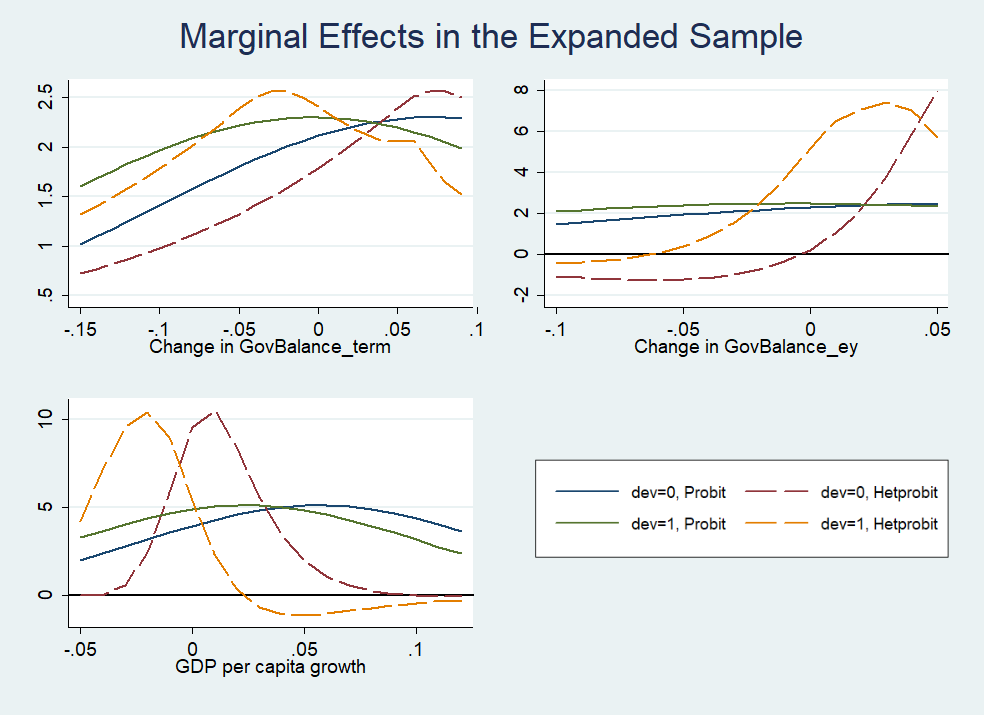
\includegraphics[width=0.8\textwidth]{AME_expanded.png}
    \end{subfigure}
    \caption{\small{Average marginal effects of the regular Probit (solid lines) and Heteroskedastic Probit model (dashed lines) for both Developed and Less Developed countries. Variables displayed are: the change in Government Balance over the leader's term, change in Government Balance in the election year and GDP per capita growth rate}}
    \label{Predicted_Expanded}
\end{figure}
